
\chapter{Formeln}

\section{Fließtext und Formeln}

\label{eq:formelnnummeriert}Formeln können in zwei Varianten geschrieben
stehen: Einmal im Text: $\mathrm{sin}(x)=\pi/3$ wie in diesem Beispiel,
oder als abgesetzte Formel: 
\[
\mathrm{sin}(x)=\pi/3
\]
Weiterhin kann man eine Formel auch automatisch nummerieren lassen:
\begin{equation}
\mathrm{sin}(x)=\pi/3\label{eq:abgesetzteformel}
\end{equation}
In dem Text kann dann auf die Gleichung (\ref{eq:abgesetzteformel})
(Achtung: Das Paket hyperref erzeugt Hyperlinks die auf der Seite
an falscher Position liegen) referenziert werden. Zwei Abgesetzte
Formeln nebeneinander können mit folgender Struktur dargestellt werden:

\begin{minipage}[t]{0.39\textwidth}%
\begin{equation}
\mathrm{e}^{\mathrm{j\,\pi}}+1=0\label{eq:allekonstentenineinergleichung}
\end{equation}
%
\end{minipage} %
\begin{minipage}[t]{0.59\textwidth}%
\begin{equation}
\mathrm{sin}(x)^{2}+\mathrm{cos}(x)^{2}=1\label{eq:trigonometrischerpythagora}
\end{equation}
%
\end{minipage} 

Alternative Darstellungsweise mit Kästchen: 

\fcolorbox{black}{white}{\begin{minipage}[t]{0.38\textwidth}%
\begin{equation}
\mathrm{e}^{\mathrm{j\,\pi}}+1=0\label{eq:allekonstentenineinergleichung-1}
\end{equation}
%
\end{minipage}}%
\fcolorbox{black}{white}{\begin{minipage}[t]{0.57\textwidth}%
\begin{equation}
\mathrm{sin}(x)^{2}+\mathrm{cos}(x)^{2}=1\label{eq:trigonometrischerpythagora-1}
\end{equation}
%
\end{minipage}}

Wenn statt der Gleichungsnummer zwei Fragezeichen erscheinen muss
häufig die Datei noch einmal übersetzt, oder label und ref haben unterschiedliche
Marken. Beim Konvertieren zwischen der .TEX-Datei und der PDF-Datei
spricht man vom sog. \textit{Setzen}.

\section{Regeln zum Formelsatz}

\label{eq:formelsatz}Für das Setzen von Formeln gibt es Regeln:
\begin{itemize}
\item Variablen werden kursiv gesetzt: $u$
\item Indizes, Konstanten, physikalische Einheiten und Funktionsnamen werden
aufrecht gesetzt: $\mathrm{kA}$
\item Zwischen Zahlenwert und Einheit wird ein kleiner Leerraum gesetzt:
$U=5\,\mathrm{V}$
\item Konstante indizes werden aufrecht gesetzt: $u_{\mathrm{min}}$
\item Variable Indizes werden kursiv gesetzt: $\overline{u}=\frac{1}{42}\sum_{k=1}^{42}u_{k}$
\item Zur Multiplikation wird der Multiplikationspunkt gesetzt: $x\cdot y=z$
\item Für das Kreuzprodukt wird das liegende Kreuz verwendet: $\boldsymbol{x}\times\boldsymbol{y}=\boldsymbol{z}$.
Weiterhin darf es für Flächenangaben verwendet werden: $A=25\,\mathrm{m}\times14\,\mathrm{m}$.
Das liegende Kreuz $\times$ ist nicht dasselbe Zeichen wie der vor-vorletzte
Buchstabe des Alphabets: x.
\item Für die Faltung wird das Sternchen verwendet: $a*b$
\item Bei Zwischenzeilen-Formeln kann statt $\mathrm{e}^{\mathrm{j}\,\varphi}$
geschrieben werden: $\mathrm{exp}\left(\mathrm{j}\,\varphi\right)$
\item Bei Zwischenzeilenformeln kann statt dem Bruch ($\frac{7}{8}$) der
Schrägstrich verwendet werden: $7/8$.
\end{itemize}
Also: $x_{\mathrm{start}}$ statt $x_{start}$, $\mathrm{sin}(x)$
statt $sin(x)$, $z=4+\mathrm{j}\,6$ statt $z=4+j\,6$, $i=4{,}5\,\mathrm{A}$
statt $i=4{,}5\,A$ und $\mathrm{e}^{\mathrm{j}\,\pi}$ statt $e^{j\,\pi}$.
Bei Zahlenwerten in Formeln sollte das Komma als Dezimaltrennzeichen
in geschweifte Klammern gesetzt werden. Damit wird ein falscher Leerraum
verhindert. Richtig: \lstinline[language=TeX]|$\pi=3{,}14$| ergibt:
$\pi=3{,}14$. Falsch: \lstinline[language=TeX]|$\pi=3,14$| ergibt:
\raisebox{-1mm}{ 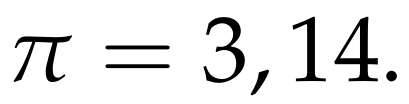
\includegraphics[width=19mm]{figures/03kommaabstand/kommaabstand}}

In Formeln kommen beispielhaft folgende Elemente vor:
\begin{itemize}
\item Wurzel: $\sqrt{\left(x\right)}$
\item n-te Wurzel: $\sqrt[3]{x}$
\item Bruch: $\frac{\text{Zähler}}{\text{Nenner}}$
\item Index: $x_{1}$
\item Index mit mehreren Buchstaben: $x_{\mathrm{start}}$
\item Sub-(sub-)Indizes: $S_{v_{\mathrm{end}_{2}}}$
\item Exponent: $x^{2}$
\item Exponent mit mehreren Buchstaben: $x^{12}$
\item Integral: $\int x^{2}\,\mathrm{d}x$ 
\item Bestimmtes Integral: $\int_{0}^{\infty}f(x)\,\mathrm{d}x$
\item Buchstaben aufrecht gesetzt (nicht kursiv): $\mathrm{x}$
\item Summenzeichen: $\sum$
\item Summenzeichen mit Grenzen: $\sum_{k=1}^{42}$
\item Griechische Buchstaben: $\alpha$, $\beta$, $\gamma$, $\theta$
\item Multiplikationspunkt (nicht: \$a{*}b\$): $a\cdot b$
\item Geschweifte Klammern unten: $\underbrace{a\cdot b}_{c}$
\item Geschweifte Klammern oben: $\overbrace{0\cdot b}^{=0}$
\item Abstand: klein (Multiplikation) $a\,b$
\item Abstand: mittel $a\ b$
\item Abstand: groß $a\quad b$
\item Doppelter großer Abstand: $a\qquad b$
\item Man achte darauf, dass nach dem Mathebefehl ein Leerzeichen steht:
$\alpha a$ \% Hinweis: \$\textbackslash alphaa\$ funktioniert nicht
\item Klammern, deren Größe sich dem Inhalt anpassen: $\left[\sqrt{x^{2}}\right]$,
$\left(\sqrt{x^{2}}\right)$, 
\item $\left|\sqrt{x^{2}}\right|$ statt $[\sqrt{x^{2}}]$, $(\sqrt{x^{2}})$,
$|\sqrt{x^{2}}|$
\item Klammern und senkrechte Striche in unterschiedlicher Größe: $\bigr)$
$\biggr)$ $\Biggr)$ $\bigl($ $\biggl($ $\Biggl($ $\bigr]$ $\biggr]$
$\Biggr]$ $\bigl[$ $\biggl[$ $\Biggl[$ $\bigr|$ $\biggr|$ $\Biggr|$ 
\item Matrix: $\left(\begin{matrix}11 & 12\\
21 & 22
\end{matrix}\right)$
\item Limes: $\lim_{x\rightarrow\infty}$ oder ${\displaystyle \lim_{x\rightarrow\infty}}$
\item Geschweifte Klammer unterhalb: $\underbrace{1+2+3}_{=6}+4$
\item Geschweifte Klammer oberhalb: $1+\overbrace{2+3+4}^{=9}$
\item Strich unterhalb: $\underline{z}$
\item Teile von Formeln können auch in unterschiedlichen Farbgebungen gesetzt
werden:\\
$\mathop{\color{blue}\sin}{\color{blue}\left({\color{brown}x}\right)^{2}+\mathop{\color{magenta}\cos}}\left(x\right)^{2}={\color{green}1}$
\item Sonderzeichen: $\smiley$
\end{itemize}
Je nach Umgebung (in-Zeile-Formel oder abgesetzte Formel) werden einige
Elemente in unterschiedlicher Größe dargestellt:$\int_{0}^{\infty}\mathrm{sin}(x)\,\mathrm{d}x$
\[
\int_{0}^{\infty}\mathrm{sin}(x)\,\mathrm{d}x
\]
In-Zeile-Formeln können in der Größe von abgesetzten Formeln gesetzt
werden: ${\displaystyle {\displaystyle \int_{0}^{\infty}\mathrm{sin}(x)\,\mathrm{d}x}}$

Latex kennt eine Vielzahl an Sonderzeichen: Erkennung von Sonderzeichen:
\url{http://detexify.kirelabs.org/classify.html} Übersicht der Sonderzeichen:
\url{http://mirrors.ctan.org/info/symbols/comprehensive/symbols-a4.pdf}

Die nachfolgende Formel ist sehr lang und wird umgebrochen:

\begin{multline*}
b_{k}=\frac{2}{T}\,\Biggl(\underbrace{\int_{-\frac{T}{2}}^{-\frac{T}{4}}-f_{3}\left(\frac{T}{2}+t\right)\,\mathrm{sin}\left(k\,\frac{2\,\pi}{T}\,t\right)\,\mathrm{d}t}_{A}+\underbrace{\int_{-\frac{T}{4}}^{0}-f_{3}\left(-t\right)\,\mathrm{sin}\left(k\,\frac{2\,\pi}{T}\,t\right)\,\mathrm{d}t}_{B}+\\
\underbrace{\int_{0}^{\frac{T}{4}}f_{3}\left(t\right)\,\mathrm{sin}\left(k\,\frac{2\,\pi}{T}\,t\right)\,\mathrm{d}t}_{C}+\underbrace{\int_{\frac{T}{4}}^{\frac{T}{2}}f_{3}\left(\frac{T}{2}-t\right)\,\mathrm{sin}\left(k\,\frac{2\,\pi}{T}\,t\right)\,\mathrm{d}t}_{D}\Biggr)
\end{multline*}

Mit der align-Umgebung kann man sehr gut Formeln untereinander setzen:

\begin{align*}
b_{k} & =\frac{2}{T}\,\left(\int_{-\frac{T}{2}}^{0}f\left(t\right)\,\mathrm{sin}\left(k\,\frac{2\,\pi}{T}\,t\right)\,\mathrm{d}t+\int_{0}^{\frac{T}{2}}-f\left(t-\frac{T}{2}\right)\,\mathrm{sin}\left(k\,\frac{2\,\pi}{T}\,t\right)\,\mathrm{d}t\right)\quad\biggl|\text{Zeitversatz}\\
 & =\frac{2}{T}\,\left(\int_{-\frac{T}{2}}^{0}f\left(t\right)\,\mathrm{sin}\left(k\,\frac{2\,\pi}{T}\,t\right)\,\mathrm{d}t-\int_{-\frac{T}{2}}^{\frac{T}{2}-\frac{T}{2}}f\left(t-\frac{T}{2}+\frac{T}{2}\right)\,\mathrm{sin}\left(k\,\frac{2\,\pi}{T}\,\left(t+\frac{T}{2}\right)\right)\,\mathrm{d}t\right)\biggl|\text{Vereinfachen}\\
 & =\frac{2}{T}\,\left(\int_{-\frac{T}{2}}^{0}f\left(t\right)\,\mathrm{sin}\left(k\,\frac{2\,\pi}{T}\,t\right)\,\mathrm{d}t-\int_{-\frac{T}{2}}^{0}f\left(t\right)\,\mathrm{sin}\left(k\,\frac{2\,\pi}{T}\,t+k\,\frac{2\,\pi}{T}\,\frac{T}{2}\right)\,\mathrm{d}t\right)\quad\biggl|\text{kürzen}\\
 & =\frac{2}{T}\,\left(\int_{-\frac{T}{2}}^{0}f\left(t\right)\,\mathrm{sin}\left(k\,\frac{2\,\pi}{T}\,t\right)\,\mathrm{d}t-\int_{-\frac{T}{2}}^{0}f\left(t\right)\,\mathrm{sin}\left(k\,\frac{2\,\pi}{T}\,t+k\,\pi\right)\,\mathrm{d}t\right)\quad\biggl|\text{kürzen}
\end{align*}


\section{Abbildungen als Gleitobjekte}

Gleitobjekte sind nicht fest im Text verankert, sondern werden durch
LaTeX so verschoben, dass der Text und die Abbildung im Idealfall
die Seite vollständig ausfüllen. Auf Abbildungen wird mit \ref{fig:plots}
verwiesen.

\begin{figure}
\hfill{}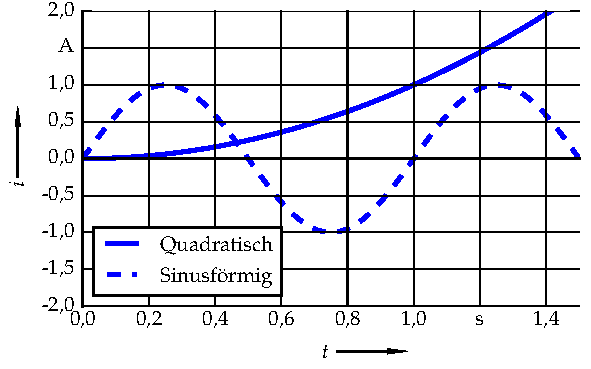
\includegraphics{figures/01plot/plotdin}\hfill{}\null

\caption{Dies ist eine Abbildung mit einer Abbildungsunterschrift, die die
Abbildung beschreibt.}
\label{fig:plots}

\end{figure}

